\documentclass{standalone}
\usepackage{tikz}
\usetikzlibrary{3d,decorations.pathmorphing,math}
\tikzset{MyPersp/.style={
scale=2,
x={(-0.2cm,-0.4cm)},
y={(   1cm,   0cm)},
z={(   0cm,   1cm)}}}

\begin{document}
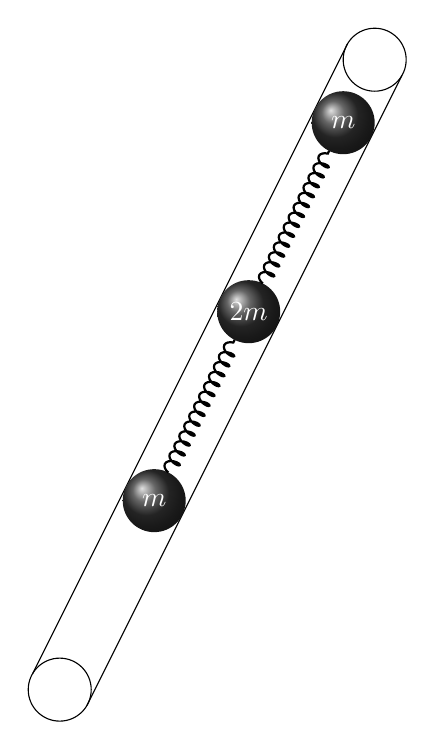
\begin{tikzpicture}[MyPersp]
\tikzmath{\xnorm = 0.447;
			  \ax=    -4;
			  \bx=    -1;
			  \cx=     2;}
\begin{scope}[canvas is yz plane at x=-5]
\draw(0,0)circle(0.2);
\end{scope}
\begin{scope}[canvas is yz plane at x=5]
\draw(0,0)circle(0.2);
\end{scope}
\draw(5, {sin(60)*0.2},-{cos(60)*0.2})--(-5, {sin(60)*0.2},-{cos(60)*0.2});
\draw(5,-{sin(60)*0.2}, {cos(60)*0.2})--(-5,-{sin(60)*0.2}, {cos(60)*0.2});
\shade[ball color=black!80, x={(1cm,0cm)},y={(0cm,1cm)}](-\ax*0.2,-\ax*0.4)circle(0.2)node{\color{white}$m$};
\shade[ball color=black!80, x={(1cm,0cm)},y={(0cm,1cm)}](-\bx*0.2,-\bx*0.4)circle(0.2)node{\color{white}$2m$};
\shade[ball color=black!80, x={(1cm,0cm)},y={(0cm,1cm)}](-\cx*0.2,-\cx*0.4)circle(0.2)node{\color{white}$m$};
\draw[thick,decorate,decoration={coil,segment length=4pt}](\bx-\xnorm,0,0)--(\xnorm+\ax,0,0);
\draw[thick,decorate,decoration={coil,segment length=4pt}](\cx-\xnorm,0,0)--(\bx+\xnorm,0,0);
\end{tikzpicture}
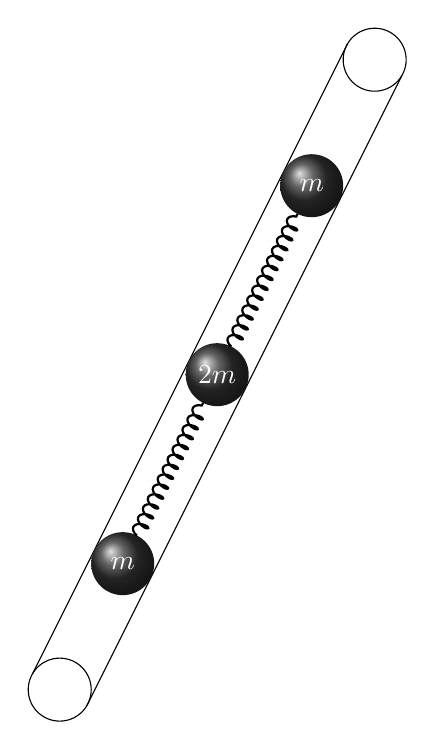
\begin{tikzpicture}[MyPersp]
\tikzmath{\xnorm = 0.447;
			  \ax=    -3;
			  \bx=     0;
			  \cx=     3;}
\begin{scope}[canvas is yz plane at x=-5]
\draw(0,0)circle(0.2);
\end{scope}
\begin{scope}[canvas is yz plane at x=5]
\draw(0,0)circle(0.2);
\end{scope}
\draw(5, {sin(60)*0.2},-{cos(60)*0.2})--(-5, {sin(60)*0.2},-{cos(60)*0.2});
\draw(5,-{sin(60)*0.2}, {cos(60)*0.2})--(-5,-{sin(60)*0.2}, {cos(60)*0.2});
\shade[ball color=black!80, x={(1cm,0cm)},y={(0cm,1cm)}](-\ax*0.2,-\ax*0.4)circle(0.2)node{\color{white}$m$};
\shade[ball color=black!80, x={(1cm,0cm)},y={(0cm,1cm)}](-\bx*0.2,-\bx*0.4)circle(0.2)node{\color{white}$2m$};
\shade[ball color=black!80, x={(1cm,0cm)},y={(0cm,1cm)}](-\cx*0.2,-\cx*0.4)circle(0.2)node{\color{white}$m$};
\draw[thick,decorate,decoration={coil,segment length=4pt}](\bx-\xnorm,0,0)--(\xnorm+\ax,0,0);
\draw[thick,decorate,decoration={coil,segment length=4pt}](\cx-\xnorm,0,0)--(\bx+\xnorm,0,0);
\end{tikzpicture}
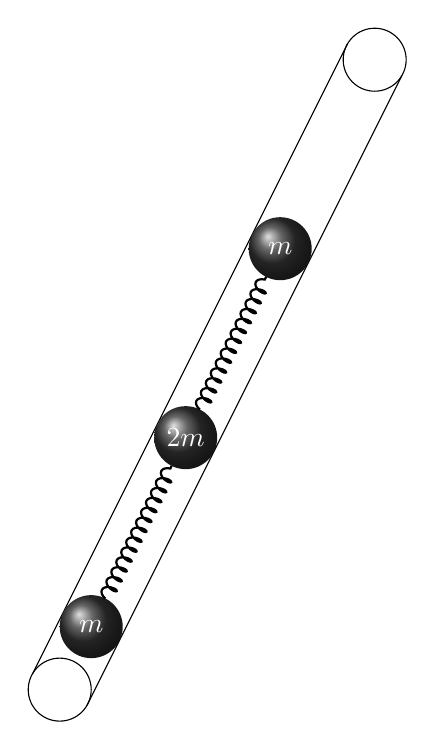
\begin{tikzpicture}[MyPersp]
\tikzmath{\xnorm = 0.447;
			  \ax=    -2;
			  \bx=     1;
			  \cx=     4;}
\begin{scope}[canvas is yz plane at x=-5]
\draw(0,0)circle(0.2);
\end{scope}
\begin{scope}[canvas is yz plane at x=5]
\draw(0,0)circle(0.2);
\end{scope}
\draw(5, {sin(60)*0.2},-{cos(60)*0.2})--(-5, {sin(60)*0.2},-{cos(60)*0.2});
\draw(5,-{sin(60)*0.2}, {cos(60)*0.2})--(-5,-{sin(60)*0.2}, {cos(60)*0.2});
\shade[ball color=black!80, x={(1cm,0cm)},y={(0cm,1cm)}](-\ax*0.2,-\ax*0.4)circle(0.2)node{\color{white}$m$};
\shade[ball color=black!80, x={(1cm,0cm)},y={(0cm,1cm)}](-\bx*0.2,-\bx*0.4)circle(0.2)node{\color{white}$2m$};
\shade[ball color=black!80, x={(1cm,0cm)},y={(0cm,1cm)}](-\cx*0.2,-\cx*0.4)circle(0.2)node{\color{white}$m$};
\draw[thick,decorate,decoration={coil,segment length=4pt}](\bx-\xnorm,0,0)--(\xnorm+\ax,0,0);
\draw[thick,decorate,decoration={coil,segment length=4pt}](\cx-\xnorm,0,0)--(\bx+\xnorm,0,0);
\end{tikzpicture}
\end{document}